To demonstrate the usefulness of the work, MLonMCU, an automatic end-to-end TinyML benchmarking tool developed by TUM EDA chair, is used. As shown in \cref{fig:evaluation_workflow}, it takes TFLite models from the MLPerf Tiny Benchmark, generates binary executables through TVM compiler with Bring Your Own Codegen (BYOC) framework and RV32IM toolchain, and run binaries on ETISS to generate instruction traces. Then, the implemented tool takes binaries and instruction traces, generating callgrind output format files. Afterwards, profiling results are visualized and evaluated by launching kcachegrind.

It is worth noticing that RISC-V vector extension and packed extension, are not used for evaluation since they are not yet supported by ETISS framework.

\begin{figure}[h]
    \centering
    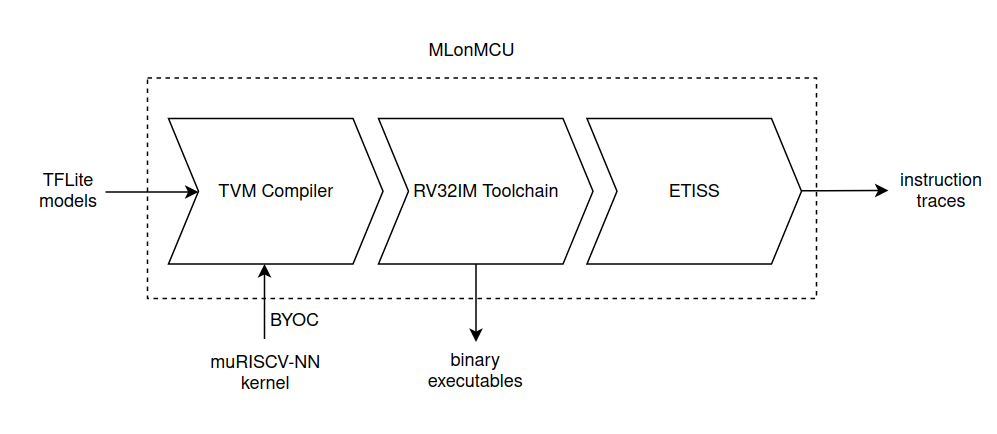
\includegraphics[width=\linewidth]{figures/evaluation_workflow.png}
    \caption{Workflow of using MLonMCU}
    \label{fig:evaluation_workflow}
\end{figure}

\section{Benchmark}
The MLPerf Tiny Benchmark Suite is used for evaluation. As introduced in \cite{banbury2021mlperf}, there are four benchmarks in the benchmark suite:

\begin{itemize}
    \item \textbf{toycar} is related to anomaly detection use case. A FC-AutoEncoder is the model. 
    \item \textbf{aww} is related to keyword spotting use case. A small depthwise-separable DNN is selected as the model.
    \item \textbf{vww} is related to visual wake words use case. MobileNetV1 is selected as the model. 
    \item \textbf{resnet} is related to image classification use case. A customized ResNet-8 is the model.
\end{itemize}

\medskip
\begin{center}
\begin{minipage}{\textwidth}
\lstset{caption={Command lines}, label=code:cmd}
\begin{lstlisting}[language=bash]
# run MLonMCU
$ python3 -m mlonmcu.cli.main flow run <benchmark> --target etiss --backend tvmaotplus
--feature-gen muriscvnnbyoc -c run.export_optional=1 -f log_instrs -c log_instrs.to_file=1 -c riscv_gcc.install_dir=<path to rv32im_ilp32> -c etiss.fpu=none -c etiss.compr
essed=0 -c etiss.atomic=0 -c mlif.debug_symbols=1

# run implemented tool
$ python3 main.py -f <ELF> -t <instruction_trace> --dump-pc=<yes/no> --dump-pos=<yes/no>

# run kcachegrind
$ OBJDUMP=<path of objdump of rv32im_ilp32 toolchain> kcachegrind <output file from implemented tool>
    
\end{lstlisting}
\end{minipage}
\end{center}

\section{Results Analysis}

As described at the beginning of this chapter, command lines for all steps are shown in \cref{code:cmd}. For each benchmark, the muRISCV-NN kernels that are spent most time on during runtime are listed in \cref{tab:benchmark_bottleneck}.

\begin{itemize}
    \item \textbf{toycar} benchmark spends time mostly in \texttt{muriscv\_nn\_vec\_mat\_mult\_t\_s8} kernel. The inner-most loop of the kernel accounts for 94.80\% of kernel instructions.
        
    \item \textbf{aww} benchmark spends time mostly in \texttt{muriscv\_nn\_mat\_mult\_nt\_t\_s8}, \texttt{muriscv \_nn\_depthwise\_conv\_3x3\_s8}, and \texttt{muriscv\_nn\_depthwise\_conv\_s8}. The inner-most loops account for 87\%, 53\% and 72\% instructions of each kernel.
    
    \item \textbf{vww} benchmark spends time mostly in \texttt{muriscv\_nn\_mat\_mult\_nt\_t\_s8}, \texttt{muriscv \_nn\_depthwise\_conv\_s8}. The inner-most loops account for 67\% and 53\% instructions of each kernel.
    
    \item \textbf{resnet} benchmark spends time mostly in \texttt{muriscv\_nn\_mat\_mult\_kernel\_s8\_s16}. The inner-most loop of the kernel accounts for 89.19\% of kernel instructions. 
\end{itemize}

\medskip
\begin{table}[h!]
    \centering
    \resizebox{\textwidth}{!}{
    \begin{tabular}{|c|c|c|c|c|}
    \hline
     benchmark & kernel & relative cost & absolute cost & calls \\
    \hline
    toycar & muriscv\_nn\_vec\_mat\_mult\_t\_s8 & 99.09 & 1,470,894 & 10 \\
    \hline
    \multirow{3}{*}{aww} & muriscv\_nn\_mat\_mult\_nt\_t\_s8 & 61.62 & 9,935,400 & 4 \\ 
    \cline{2-5}
    & muriscv\_nn\_depthwise\_conv\_3x3\_s8 & 23.09 & 3,723,793 & 4 \\
    \cline{2-5}
    & muriscv\_nn\_depthwise\_conv\_s8 & 14.84 & 2,392,755 & 1 \\
    \hline
    \multirow{2}{*}{vww} & muriscv\_nn\_mat\_mult\_nt\_t\_s8 & 68.64 & 31,640,050 & 13 \\ 
    \cline{2-5}
    & muriscv\_nn\_depthwise\_conv\_3x3\_s8 & 23.48 & 10,823,587 & 13 \\
    \hline
    \multirow{2}{*}{resnet} & muriscv\_nn\_mat\_mult\_kernel\_s8\_s16 & 89.19 & 48,640,732 & 2016 \\
    \cline{2-5}
    & muriscv\_nn\_q7\_to\_q15\_with\_offset & 5.43 & 2,959,014 & 31266 \\
    \hline
    \end{tabular}
    }
    \caption{Kernels that account for more than 5\% of total instructions of each benchmark. Cost refers to instruction counts. Relative cost equals absolute cost divided by total number of instructions of specified benchmark.}
    \label{tab:benchmark_bottleneck}
\end{table}

\medskip
\begin{table}[h!]
    \centering
    \resizebox{\textwidth}{!}{
    \begin{tabular}{|c|c|c|c|}
    \hline
    benchmark & kernel & bottleneck(rel) & bottleneck(abs) \\
    \hline
    toycar & muriscv\_nn\_vec\_mat\_mult\_t\_s8 & 94.80\% & 1,394,076 \\
    \hline
    \multirow{3}{*}{aww} & muriscv\_nn\_mat\_mult\_nt\_t\_s8 & 86.98\% & 8,642,304 \\
    \cline{2-4}
    & muriscv\_nn\_depthwise\_conv\_3x3\_s8 & 52.80\% & 1,966,380 \\ 
    \cline{2-4}
    & muriscv\_nn\_depthwise\_conv\_s8 & 78.28\% & 1,872,955 \\
    \hline
    \multirow{2}{*}{vww} & muriscv\_nn\_mat\_mult\_nt\_t\_s8 & 67.50\% & 21,362,944 \\
    \cline{2-4}
    & muriscv\_nn\_depthwise\_conv\_3x3\_s8 & 53.20\% & 5,754,537 \\ 
    \hline
    \multirow{2}{*}{resnet} & muriscv\_nn\_mat\_mult\_kernel\_s8\_s16 & 93.20\% & 45,434,368 \\
    \cline{2-4}
    & muriscv\_nn\_q7\_to\_q15\_with\_offset & 98.91\% & 2,926,848 \\ 
    \hline
    \end{tabular}
    }
    \caption{Bottleneck in kernel. \textbf{bottleneck(abs)} refers to instruction counts of bottleneck part, whereas \textbf{bottleneck(rel)} is \textbf{bottleneck(abs)} divided by total number of instructions of the kernel.}
    \label{tab:muriscv_nn_bottleneck}
\end{table}

\subsection{Possible Optimization Options}
Thanks to kcachegrind, machine code and corresponding source code annotations of bottleneck parts inside critical kernels for each benchmark are available. This enables us to analyze those critical parts directly and to figure out suitable optimization strategies.

It is worth noticing that the quantitative results of instruction counts reduction with each optimization is based on hypothetical estimation. Namely, by looking at machine code and source code annotations side by side in kcachegrind, it is explicit to observe instructions that can be merged or removed and to reason about the numbers.

\subsubsection{Multiply-Accumulate Instruction}
Taking \texttt{muriscv\_nn\_mat\_mult\_nt\_t\_s8} kernel of aww benchmark for example, source line 522, 523, 526, and 527 do multiply-accumulate operations. Multiply-and-accumulate operations in RISC-V P extension are capable of combining \texttt{mul} and \texttt{add} into single instruction. This results in a reduction of 23.5\% of instructions in the critical part (inner-most loop) of the kernel. Results of all kernels concerned are listed in \cref{tab:mac_improvement}.

\begin{figure}[ht]
    \centering
    \begin{minipage}{0.45\textwidth}
        \centering
        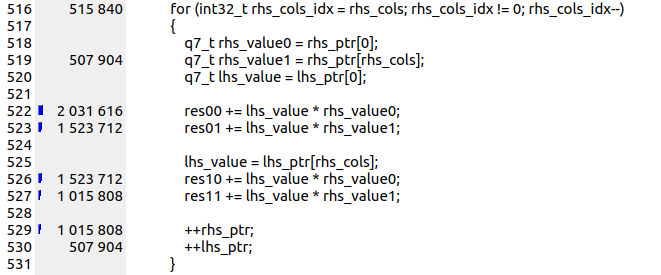
\includegraphics[width=\textwidth]{figures/aww_bottleneck_source_1.png}
    \end{minipage}\hfill
    \begin{minipage}{0.54\textwidth}
        \centering
        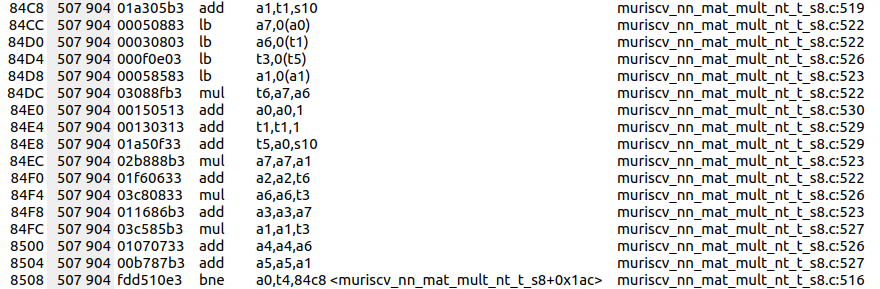
\includegraphics[width=\textwidth]{figures/aww_bottleneck_assembly_1.png}
    \end{minipage}
    \caption{Bottleneck inside \texttt{muriscv\_nn\_mat\_mult\_nt\_t\_s8} kernel for aww benchmark}
    \label{fig:aww_bottleneck}
\end{figure}

\medskip
\begin{table}[h!]
    \centering
    \resizebox{\textwidth}{!}{
    \begin{tabular}{|c|c|c|c|c|}
    \hline
     benchmark & kernel & original & with MAC & reduction \\
    \hline
    toycar & muriscv\_nn\_vec\_mat\_mult\_t\_s8 & 1,394,076 & 1,133,100 & -18.7\% \\
    \hline
    \multirow{3}{*}{aww} & muriscv\_nn\_mat\_mult\_nt\_t\_s8 & 8,642,304 & 6,610,688 & -23.5\% \\ 
    \cline{2-5}
    & muriscv\_nn\_depthwise\_conv\_3x3\_s8 & 1,966,380 & 1,927,980 & -1.95\% \\
    \cline{2-5}
    & muriscv\_nn\_depthwise\_conv\_s8 & 1,872,955 & 1,602,235 & -13.38\% \\
    \hline
    \multirow{2}{*}{vww} & muriscv\_nn\_mat\_mult\_nt\_t\_s8 & 21,362,944 & 15,268,096 & -28.5\% \\ 
    \cline{2-5}
    & muriscv\_nn\_depthwise\_conv\_3x3\_s8 & 5,754,537 & 5,659,305 & -1.65\% \\
    \hline
    \multirow{2}{*}{resnet} & muriscv\_nn\_mat\_mult\_kernel\_s8\_s16 & 45,434,368 & 32,933,376 & -27.51\% \\
    \cline{2-5}
    & muriscv\_nn\_q7\_to\_q15\_with\_offset & 2,926,848 & - & - \\
    \hline
    \end{tabular}
    }
    \caption{Instructions reduction in critical part of each kernel with MAC }
    \label{tab:mac_improvement}
\end{table}


\subsubsection{Post-Incrementing Load/Store}
Post-incrementing load/store instructions perform memory access and increment memory address stored in register by a given offset afterwards. Taking \texttt{muriscv\_nn\_q7\_to \_q15\_with\_offset} kernel in resnet benchmark for example, \texttt{lb a5,0(a0)} and \texttt{add a0,a0,1} can be merged into a single post-incrementing load instruction. Also, \texttt{add a1,a1,2} and \texttt{sh a5,-2(a1)} can be merged into a single post-incrementing store instruction. This results in a reduction of 20.64\% of instructions in the critical part (while-loop) of the kernel. Results of all kernels concerned are listed in \cref{tab:post_increment_improvement}.

\begin{figure}[ht]
    \centering
    \begin{minipage}{0.35\textwidth}
        \centering
        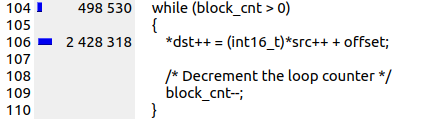
\includegraphics[width=\textwidth]{figures/resnet_bottleneck_source_2.png}
    \end{minipage}\hfill
    \begin{minipage}{0.65\textwidth}
        \centering
        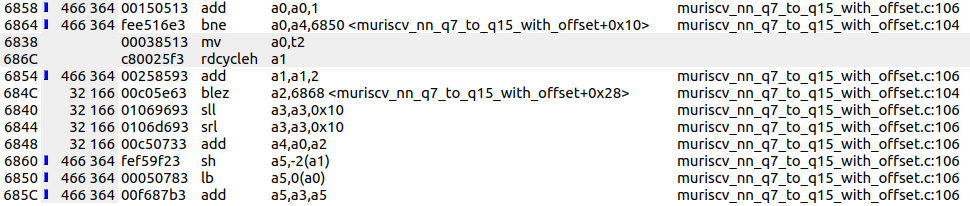
\includegraphics[width=\textwidth]{figures/resnet_bottleneck_assembly_2.png}
    \end{minipage}
    \caption{\texttt{muriscv\_nn\_q7\_to\_q15\_with\_offset} kernel in resnet benchmark}
    \label{fig:resnet_post_increment_example}
\end{figure}

\medskip
\begin{table}[h!]
    \centering
    \resizebox{\textwidth}{!}{
    \begin{tabular}{|c|c|c|c|c|}
    \hline
     benchmark & kernel & original & with post-increment ld/st & reduction \\
    \hline
    toycar & muriscv\_nn\_vec\_mat\_mult\_t\_s8 & 1,394,076 & 1,046,108 & -24.96\% \\
    \hline
    \multirow{3}{*}{aww} & muriscv\_nn\_mat\_mult\_nt\_t\_s8 & 8,642,304 & 7,626,496 & -11.75\% \\ 
    \cline{2-5}
    & muriscv\_nn\_depthwise\_conv\_3x3\_s8 & 1,966,380 & * & * \\
    \cline{2-5}
    & muriscv\_nn\_depthwise\_conv\_s8 & 1,872,955 & * & * \\
    \hline
    \multirow{2}{*}{vww} & muriscv\_nn\_mat\_mult\_nt\_t\_s8 & 21,362,944 & 18,315,520 & -17.27\% \\ 
    \cline{2-5}
    & muriscv\_nn\_depthwise\_conv\_3x3\_s8 & 5,754,537 & * & * \\
    \hline
    \multirow{2}{*}{resnet} & muriscv\_nn\_mat\_mult\_kernel\_s8\_s16 & 45,434,368 & 36,058,624 & -20.64\% \\
    \cline{2-5}
    & muriscv\_nn\_q7\_to\_q15\_with\_offset & 2,926,848 & 1,994,120 & -31.87\% \\
    \hline
    \end{tabular}
    }
    \caption{Instructions reduction in critical part of each kernel with post-incrementing load/store. * means it is difficult to estimate the number hypothetically since for-loop bodies are much more complicated.}
    \label{tab:post_increment_improvement}
\end{table}

\subsubsection{Hardware Loop}
Hardware loop is capable of removing branching and the update of counters and achieves zero-overhead. Taking \texttt{muriscv\_nn\_q7\_to \_q15\_with\_offset} kernel in resnet benchmark for example, \texttt{add a0,a0,1} and \texttt{bne a0,a4,6850} can be replaced with a single hardware loop setup instruction, resulting in a reduction of 31.87\% in the critical part (while-loop) of the kernel. Results of all kernels concerned are listed in \cref{tab:hardware_loop_improvement}.

\medskip
\begin{table}[ht!]
    \centering
    \resizebox{\textwidth}{!}{
    \begin{tabular}{|c|c|c|c|c|}
    \hline
     benchmark & kernel & original & with hardware loop & reduction \\
    \hline
    toycar & muriscv\_nn\_vec\_mat\_mult\_t\_s8 & 1,394,076 & 1,220,092 & -12.48\% \\
    \hline
    \multirow{3}{*}{aww} & muriscv\_nn\_mat\_mult\_nt\_t\_s8 & 8,642,304 & 7,626,497 & -11.75\% \\ 
    \cline{2-5}
    & muriscv\_nn\_depthwise\_conv\_3x3\_s8 & 1,966,380 & * & * \\
    \cline{2-5}
    & muriscv\_nn\_depthwise\_conv\_s8 & 1,872,955 & * & * \\
    \hline
    \multirow{2}{*}{vww} & muriscv\_nn\_mat\_mult\_nt\_t\_s8 & 21,362,944 & 18,315,521 & -17.27\% \\ 
    \cline{2-5}
    & muriscv\_nn\_depthwise\_conv\_3x3\_s8 & 5,754,537 & * & * \\
    \hline
    \multirow{2}{*}{resnet} & muriscv\_nn\_mat\_mult\_kernel\_s8\_s16 & 45,434,368 & 42,309,121 & -6.88\% \\
    \cline{2-5}
    & muriscv\_nn\_q7\_to\_q15\_with\_offset & 2,926,848 & 1,994,121 & -31.87\% \\
    \hline
    \end{tabular}
    }
    \caption{Instructions reduction in critical part of each kernel with hardware loop support. * means it is difficult to estimate the number hypothetically since the for-loop bodies are much more complicated.}
    \label{tab:hardware_loop_improvement}
\end{table}

\subsubsection{Combination of Three Optimizations}
As shown in \cref{tab:total_improvement}, the combination of these three optimizations results in a reduction of instructions around 50\% for matrix-multiply specific kernels. For depthwise specific kernels, it is difficult to provide hypothetical estimations because of the complicated loop structures.

\medskip
\begin{table}[ht!]
    \centering
    \resizebox{\textwidth}{!}{
    \begin{tabular}{|c|c|c|c|c|}
    \hline
     benchmark & kernel & original & all three combined & reduction \\
    \hline
    toycar & muriscv\_nn\_vec\_mat\_mult\_t\_s8 & 1,394,076 & 698,141 & -49.92\% \\
    \hline
    \multirow{3}{*}{aww} & muriscv\_nn\_mat\_mult\_nt\_t\_s8 & 8,642,304 & 5,086,977 & -41.14\% \\ 
    \cline{2-5}
    & muriscv\_nn\_depthwise\_conv\_3x3\_s8 & 1,966,380 & * & * \\
    \cline{2-5}
    & muriscv\_nn\_depthwise\_conv\_s8 & 1,872,955 & * & * \\
    \hline
    \multirow{2}{*}{vww} & muriscv\_nn\_mat\_mult\_nt\_t\_s8 & 21,362,944 & 10,696,961 & -49.93\% \\ 
    \cline{2-5}
    & muriscv\_nn\_depthwise\_conv\_3x3\_s8 & 5,754,537 & * & * \\
    \hline
    \multirow{2}{*}{resnet} & muriscv\_nn\_mat\_mult\_kernel\_s8\_s16 & 45,434,368 & 21,995,009 & -51.59\% \\
    \cline{2-5}
    & muriscv\_nn\_q7\_to\_q15\_with\_offset & 2,926,848 & 1,994,121 & -31.87\% \\
    \hline
    \end{tabular}
    }
    \caption{Instructions reduction in critical part of each kernel with three optimizations combined. * means it is difficult to estimate the number hypothetically since the for-loop bodies are much more complicated.}
    \label{tab:total_improvement}
\end{table}



